\documentclass[a4paper, parskip=half]{scrartcl}
%\documentclass[a4paper, parskip=half]{scrartcl}
\usepackage[utf8]{inputenc}
\usepackage[T1]{fontenc}
\usepackage[english, ngerman]{babel}
%\usepackage{libertine}
\usepackage{xstring}
\usepackage{amssymb,amstext,amsmath}
\usepackage{graphicx}
\usepackage{sectsty}
\usepackage{multirow}
\usepackage{dsfont}
\usepackage{amsfonts}
\usepackage{graphics}
\usepackage{float}
\usepackage{dsfont}
\usepackage[hidelinks]{hyperref}
\usepackage{caption}
\usepackage{ifthen}
\usepackage[table]{xcolor}
\usepackage{booktabs}

\newcommand{\myMail}[1]{\href{mailto:#1}{#1}}

\newcommand{\myImage}[3][\textwidth]{
  \begin{center}
    \begin{minipage}{\linewidth}
      \centering 
      \makebox[0cm]{\includegraphics[width=#1]{#2}}
      \ifthenelse{ \equal{#3}{}} {
      
      } {
        \captionof{figure}{#3}
        %% \label{#3}
      }
    \end{minipage}
   
  \end{center}
}

\newcommand{\myTitlepage}{%
\begin{titlepage}
  \begin{center}
    \vspace{5cm}
    \huge\bfseries
    \myTitle
    \vspace{1cm}

    \large\normalfont von

    \bigskip
    \textbf{\myAuthor}

    \myDate

    \vspace{1cm}
    
    \large\normalfont
    Versuchsdurchführung am

    \textbf{\exDate}
    \vspace{1cm}
    
    Dozent

    \textbf{\exDoc}
    
    
    \myImage[10cm]{\myTitleImage}{}
  \end{center}
  \vfill
  \enlargethispage{2cm}
  \parbox[t]{0.55\textwidth}{%
   \myTitleLeft
  }
  \parbox[t]{0.45\textwidth}{\raggedleft%
    \myTitleRight
  }
\end{titlepage}
}

\newcommand{\mySecRef}[1]{%
  \hyperref[sec:#1]{Punkt-}\ref{sec:#1}%
}


\newcommand{\myPackage}[1]{%
  \textit{#1}-Paket%
}

\newcommand{\myFormat}[1]{%
  \textit{#1}%
}

\newcommand{\myPath}[1]{%
  \textit{#1}%
}

\newcommand{\myTitle}{Ba 6: Physik und Technik des Helium-Neon-Lasers}
\newcommand{\myAuthor}{Artem Gerassimoff, Alexander Heinisch, Dominik Wille}
\newcommand{\myDate}{\today}
\newcommand{\exDate}{06.11.2013 10-14 Uhr}
\newcommand{\exDoc}{Patryk Kusch}
\newcommand{\myTitleImage}{img/HNL0}
\newcommand{\myTitleLeft}{%
   \textbf{Freie Universität Berlin}\\
   Fachbereich Physik\\
   Physikalisches Fortgeschrittenenpraktikum%
}
\newcommand{\myTitleRight}{%
  \textbf{Kontaktadressen:}\\
  \myMail{dominik.wille@fu-berlin.de} \\
  \myMail{matthias.heinisch@gmx.de} \\
  \myMail{art.geras@gmail.com}
}

\begin{document}
\myTitlepage
\tableofcontents
\newpage

%\input{einführung}

\newpage

\section{Aufgaben}
\subsection{Aufgabe 1}
Inbetriebnahme des NaJ-Detektors (Hochspannung wird vom Assistenten eingestellt). Betrachten der Impulsformen ($^{137}$Cs-Quelle) vor und hinter dem Hauptverstärker; Skizze der Impulsformen ins Protokoll (Achsenbeschriftung!); Bestimmung der Anstiegs-und Abfallzeiten der Impulse; Diskussion.

\subsection{Aufgabe 2}
Energieeichung des NaJ-Detektors mit $^{60}$Co, $^{22}$Na, $^{137}$Cs und Bestimmung der Energieauflösung für alle Photopeaks. Dabei ist die Verstärkung am Hauptverstärker so einzustellen, dass der Photopeak der 1.33 MeV $^{60}$Co-Linie im Konversionsbereich des VKA liegt. Bestimmung der Peaklagen und Halbwertsbreiten direkt am Rechner (Cursor, Fehler 
abschätzen!). Messpunkte und Eichgerade auf Millimeterpapier darstellen. 

\subsection{Aufgabe 3}
Bestimmung des Massenschwächungskoeffizienten von Pb, Cu und Al für die 1.33 MeV $^{60}$Co-Linie. Hierzu die starke $^{60}$Co-Quelle (wird vom Assistenten eingesetzt), Kollimator und NaJ-Detektor verwenden. Die Zählrate wird durch Integration über den Photopeak direkt am Rechner bestimmt (Festlegen einer Region of Interest(ROI), Zeitvorwahl, Totzeit 
beachten!). Graphische Darstellung der Zählrate über der Absorberdicke parallel zur Messung. 

\subsection{Aufgabe 4}
Inbetriebnahme des Ge-Detektors (Hochspannung wird vom Assistenten eingestellt). Protokollieren der Impulsformen vor und nach dem Hauptverstärker, Bestimmung der Anstiegs- und Abfallzeiten der Impulse.

\subsection{Aufgabe 5}
Energieeichung des Ge-Detektors mit $^{60}$Co (Verstärkung wie in 2. abgleichen), $^{22}$Na, $^{137}$Cs, $^{241}$Am, und Bestimmung der Energieauflösung für alle Photopeaks. Aufnahme eines $^{60}$Co-Spektrums mit guter Statistik, grafische Ausgabe und quantitative Diskussion 
(Bestimmung von Compton-Kanten, "Back-Scatter"-Linien, “Escape"-Linien; Vergleich mit berechneten Werten). 

\subsection{Aufgabe 6}
Bestimmung der Röntgenkonversionsline von $^{133}$Ba (E ~ 30 keV) über die kritische Absorption (Ge-Detektor). Als Absorber sind Sn, Sb, Te und J verfügbar. Um Einflüsse der Geometrie und der Absorberdicke auf die absolute Zählrate zu kontrollieren und zu eliminieren, sollte die 81-keV-Linie als Referenz genutzt werden. Die Messgrößen (Zählrate im interessierenden Peak bzw. Verhältnis dieser Zählrate zur Referenzzählrate) sind grafisch über der Lage der Absorptionskante für den entsprechenden Absorber darzustellen.

\newpage

\section{Durchführung und Auswertung}

\subsection{Aufgabe 1 - Einschalten des Versuchsaufbaus}
Die Geräte wurde von unserem Versuchsleiter eingeschaltet und er wies uns in die Funktionsweise der Geräte ein. Danach stellten wir die Spannungen $U_{FR}$, $U_{KA}$ und $U_{FA}$ auf die folgenden Werte ein:

\begin{tabular}{l l l}
$U_{FR}$ & = $113\pm 2$ V & (Beschleunigungsspannung)\\
$U_{KA}$ & = 0V & (Glühkathode)\\
$U_{FA}$ & = $106\pm 0,5$V & (Massenfilters)\\
\end{tabular}

Diese Werte wurden während der folgenden Messung nicht mehr verändert. 
Es gelang uns, den Druck während den Messungen konstant zu halten. Da auch bei mehreren Messungen des selben Gases keine Schwankungen des m/q-Wertes auftraten, nahmen wir diesen Fehler als vernachlässigbar klein an und wird in der folgenden Auswertung nicht berücksichtigt.

\subsection{Restgas-Messung}
Bei dieser Messung machten wir uns mit dem Programm LabView vertraut und stellten die Verstärkung auf $10^{-10}$. Der Druck betrug dabei $8,9 \cdot 10^{-6}$ mbar. Zudem schlossen wir Ventil V3, öffneten das Ventil V4 und nahmen mehrere Messungen von dem Restgas. In Abb. 7 und in Tab. 1 werden die gemittelten Ergebnisse dieser Messungen dargestellt.\\
Aus [4] wissen wir, dass der Peak bei m/q=18 für den Wasseranteil in dem Gas steht. Das liegt daran, dass in dem Rezipienten immer ein geringer Wasseranteil vorhanden ist, der sich, wenn das Gerät ausgeschaltet ist, auf der Glühkathode niederschlägt.

\myImage[9cm]{img/RGbalk}{Überarbeitete Daten aus der Restgasmessung}

\begin{center}
\begin{tabular}{c|c|c}
m/q [u/e] & p [$10^{-7} mbar$] & Ionen\\	
\hline	
12,5 &	0,16 & - \\
14,5 &	0,26 & $N_2$\\
16,4 &	2,20 & $O_2$\\
17,3 &	15,09 & $H_2O$\\
18,3 &	59,33 & $H_2O$ Peak\\
20,3 &	0,49 & Argon\\
26,3 &	0,73 & Ethanol\\
27,3 &	1,19 & Ethanol\\
28,2 &	8,33 & $N_2$ Peak\\
31,3 &	0,59 & Ethanol Peak\\
32,2 &	0,15 & $O_2$ Peak\\
42,2 &	0,48 & $CO_2$ Peak\\
\end{tabular}
\end{center}
\captionof{table}{Ergebnisse der Messung von dem Restgas bei einem Druck von $8,9\cdot 10^{-6}mbar$ mit errechneten Partialdrücke p und Zuordnung zu Ionen}

\subsection{Testgas 1 - Dosierung und Messung}
Über das Ventil V1A-D wurde das Testgas (in diesem Fall Argon) in die Vorkammer gelassen bis die Nadel am Druckmessgerät einmal kurz ausschlug. Anschließend öffneten wir das Ventil V2 und das Dosierventil vorsichtig, damit das Gas in den Rezipienten gelangen konnte. Nun stellten wir den Emissionsstrom der Glühkathode auf 0,2 mA, warteten kurz und notierten den Druck im Rezipienten. Anschließend starteten wir am PC das Messprogramm. Als dieses fertig war, schlossen wir das Ventil V4 und Dosierventil und öffneten vorsichtig das Ventil V3. Wir warteten anschließend 10 Minuten, bis die Vorpumpe den Rezipienten wieder leerte. Diesen Vorgang wiederholten wir für die Messung von Testgas 2 und 3.\\
Um die Messdaten auszuwerten, änderten wir die Vorzeichen der Häufigkeiten und stellten die Graphen durch Balken dar. Anschließend berechneten wir die lokalen Maxima und den Partialdruck der entsprechenden Ionen. Die Zuordnung zu den Ionen erfolgte durch [4]. Die Ergebnisse sind in Abb. 8 und in Tab. 2 dargestellt:\\

\myImage[9cm]{img/AGbalk}{Massenspektrum von Argon}

\begin{center}
\begin{tabular}{c|c|c}
m/q [u/e] & p [$10^{-7} mbar$] & Ionen\\	
\hline	
2,6 & 0,03	&\\	
14,0 & 0,18	&\\	
14,8 & 0,21	&\\	
16,4 & 0,50	&\\	
17,3 & 4,39	&\\	
18,3 & 17,71 & $H_2O$ Peak\\
20,3 & 0,42	& Argon\\
25,7 & 0,20	&\\
26,8 & 0,17	&\\
28,3 & 2,11	& $N_2$ Peak\\
40,2 & 11,51 & Argon Peak\\
42,2 & 0,16	&\\
43,3 & 0,06	&\\
44,2 & 0,19	&\\
58,3 & 0,18	&\\
\end{tabular}
\end{center}
\captionof{table}{Ergebnisse der Messung von Argon bei einem Druck von $4\cdot 10^{-6}mbar$ mit errechneten Partialdrücke p und Zuordnung zu Ionen}

\subsection{Testgas 2, 3 und Luft - Dosierung und Messung}
Bei der Messung dieser Gase sind wir wie oben beschrieben vorgegangen. Die Ergebnisse dieser Messungen werden in den folgenden Abbildungen 9, 10 und 11, sowie in den Tabellen 3, 4 und 5 dargestellt.

\myImage[9cm]{img/ACbalk}{Massenspektrum von Aceton}

\begin{center}
\begin{tabular}{c|c|c}
m/q [u/e] & p [$10^{-7} mbar$] & Ionen\\	
\hline	
2,9 &	0,77 &\\
13,0 &	0,28 &\\
14,4 &	0,97 & Aceton\\
16,4 &	2,25 &\\
17,3 &	5,84 & $H_2O$\\
18,3 &	23,09 & $H_2O$ Peak\\
21,7 &	0,35 & Argon\\
26,3 &	0,80 & Aceton\\
27,3 &	0,90 & Aceton\\
28,3 &	11,22 & Aceton, $N_2$ Peak\\
29,9 &	0,077 & Aceton\\
30,8 &	0,28 &\\
31,7 &	0,22 &\\
39,3 &	0,23 & Aceton\\
39,8 &	0,18 & Argon Peak\\
41,3 &	0,22 & Aceton\\
42,3 &	0,41 & Aceton\\
43,3 &	6,57 & Aceton Peak\\
44,1 &	0,95 &\\
45,0 &	0,24 &\\
45,9 &	0,35 &\\
58,3 &	0,80 &\\
\end{tabular}
\end{center}
\captionof{table}{Ergebnisse der Messung von Aceton bei einem Druck von $5,7\cdot 10^{-6}mbar$ mit errechneten Partialdrücke p und Zuordnung zu Ionen}

\myImage[10cm]{img/ETHbalk}{Massenspektrum von Ethanol}

\begin{center}
\begin{tabular}{c|c|c}
m/q [u/e] & p [$10^{-7} mbar$] & Ionen\\	
\hline	
2,6 &	0,17 &\\
14,4 &	0,64 & Ethanol\\
15,4 &	3,04 & Ethanol\\
16,4 &	1,90 &\\
17,4 &	5,56 & $H_2O$\\
18,4 &	22,11 & $H_2O$ Peak\\
20,0 &	0,24 &\\
24,7 &	0,38 & Ethanol\\
26,3 &	0,57 & Ethanol\\
27,3 &	0,66 & Ethanol\\
28,3 &	9,09 & Ethanol\\
30,1 &	0,16 & Ethanol\\
30,7 &	0,33 & Ethanol\\
31,7 &	0,327 & Ethanol Peak\\
39,8 &	0,25 &\\
41,3 &	0,13 &\\
42,3 &	0,31 & Ethanol\\
43,3 &	5,90 & Ethanol\\
44,1 &	0,84 & Ethanol\\
45,8 &	0,39 & Ethanol\\
\end{tabular}
\end{center}
\captionof{table}{Ergebnisse der Messung von Ethanol bei einem Druck von $5,0\cdot 10^{-5}mbar$ mit errechneten Partialdrücke p und Zuordnung zu Ionen}

\myImage[10cm]{img/Luftbalk}{Massenspektrum von Luft}

\begin{center}
\begin{tabular}{c|c|c}
m/q [u/e] & p [$10^{-7} mbar$] & Ionen\\	
\hline	
2,6 &	0,20 &\\
14,4 &	1,41 & $N_2$\\
15,0 &	0,08 &\\
16,4 &	1,62 & $O_2$\\
17,3 &	5,31 & $H_2O$\\
18,3 &	17,71 & $H_2O$ Peak\\
19,8 &	0,20 &\\
25,5 &	0,29 &\\
27,4 &	0,48 &\\
28,2 &	26,52 & $N_2$ Peak\\
30,2 &	0,39 & $N_2$\\
30,8 &	0,15 &\\
40,2 &	0,13 & $O_2$ Peak\\
40,8 &	0,23 &\\
42,0 &	0,23 &\\
42,6 &	0,28 &\\
44,2 &	0,48 &\\
\end{tabular}
\end{center}
\captionof{table}{Ergebnisse der Messung von Luft bei einem Druck von $5,6\cdot 10^{-6}mbar$ mit errechneten Partialdrücke p und Zuordnung zu Ionen}

\newpage
\subsection{Auflösungsvermögen des Spektrometers}
Aus Gl. 8 ist bekannt:

\begin{equation}
\notag
b = \frac{2qV}{mr_{0}^{2}\omega^{2}}
\end{equation}

Daraus folgt für m:

\begin{equation}
m = \frac{2qV}{br_{0}^{2}\omega^{2}}
\end{equation}

Wenn wir nun zwei Punkte auf der Arbeitsgeraden haben, ergibt sich bei einer konstanten Spannung die Breite des Massenpeaks:

\begin{equation}
\Delta m = \frac{2qV}{r_{0}^{2}\omega^{2}}\cdot \left( \frac{1}{b_1}-\frac{1}{b_2}\right) \qquad \text{mit} \qquad b_1 < b_2
\end{equation}

Nehmen wir nun an, dass sich die gemessenen Massen in der Mitte der Peaks befindet, dann gilt für b:

\begin{equation}
b = \frac{b_1 + b_2}{2}
\end{equation}

Daraus folgt:

\begin{equation}
\frac{b_1 + b_2}{2}=\frac{2qV}{mr_0^2 \omega^2} \leftrightarrow m = \frac{2qV}{r_0^2 \omega^2}\cdot \frac{2}{b_1 + b_2}
\end{equation}

Und somit für m/$\Delta$ m:

\begin{equation}
\frac{m}{\Delta m} = \frac{2}{(b_1+b_2)\cdot \left(\frac{1}{b_1}-\frac{1}{b_2}\right)} = \frac{2}{\frac{b_2}{b_1}-\frac{b_1}{b_2}} = \text{const.}
\end{equation}

Geht man davon aus, dass $\Delta$m mit der Beschleunigungsspannung zusammenhängt, ergibt sich für Ionen im Filter eine Geschwindigkeit von:

\begin{equation}
v=\sqrt{\frac{2qU_B}{m}}
\end{equation}

Je höher die Beschleunigungsspannung ist, desto kürzer ist die Aufenthaltsdauer im Massenfilter und desto geringer ist die Genauigkeit. Daraus folgt für die Anzahl $n$ der Durchlaufenen Schwingungen:

\begin{equation}
n = \frac{f\cdot l}{v}= f\cdot l \cdot \sqrt{\frac{m}{2qU_B}}
\end{equation}

mit der Frequenz $f$ und der Länge $l$ des Massenfilter.\\
Es wurden zwei Messungen mit Luft als Testgas durchgeführt, um diese Relationen zu untersuchen. Dabei variierte bei der ersten Messung der Wert von $a$ und bei der Zweiten der Wert von $U_{FA}$.

\myImage[10cm]{img/VAR}{Messung des Massenspektrums für Luft unter Variation der Auflösung a}
\subsection{Aufgabe 2 - Justierlaserleistung und Transmission der Spiegel}

Die Messung der Justierlaserleistung wurde von uns durch den vorgegebenen Bandpassfilter von 633 nm durchgeführt. Die Fehler wurden auf $\pm$ 50 $\mu$W geschätzt, da keine Beschreibung des Messgeräts zu finden war. Die gemessene Leistung betrug:

\begin{equation}
P = (500 \pm 50) \mu W
\end{equation}

Die Messung der Transmission der Spiegel haben wir für jeden Spiegel getrennt durchgeführt. Die Messungen ergaben folgende Werte:

- Für den planaren Spiegel S2:

\begin{equation}
I_{2} = (0.50 \pm 0.05) \mu W
\end{equation}

- Für den Hohlspiegel S1:

\begin{equation}
	I_{2} = (0.55 \pm 0.05) \mu W
\end{equation}

Wie man sieht, entsprechen die Werte den erwarteten Werten von $\approx$ 0,1\%. Die Transmission wird durch 

\begin{align}
	T &= \frac{I_{T}}{I_{0}} \\
	T_{1} &= (0.11 \pm 0.015)\% \\
	T_{2} &= (0.10 \pm 0.014)\% 
\end{align}

berechnet. Die Fehler wurden mit Hilfe der Gaußsche Fehlerfortpflanzung ausgerechnet.

Die Polarisationsmessung war sehr ungenau. Wir hatten keine Möglichkeit den Polarisationsfilter zu fixieren. Also mussten wir den Filter in der Hand so ruhig wie möglich halten und die Messung durchführen. Unsere Messung ergab ein Maximum der Intensität bei $(1 \pm 2)^{\circ}$.

%%% TeX-master: ''hene.tex''
\subsection{Aufgabe 3}
Die Modenstruktur des Justierlasers kann dafür herangezogen werden um die ideale Resonatorlänge zu bestimmen. Es gilt:
\begin{align}
k &= \frac{2\pi}{\lambda}  = \frac{n\pi}{d} \\
\Rightarrow \Delta f &= \frac{c}{\lambda} = \frac{c}{2d} \\
\Rightarrow d &= \frac{c}{2\Delta f}
\end{align}
\myImage[10cm]{img/55}{Modenspecktrum des Justierlasers}
Gemessen wurde bei einer Frequenz von $f = 2\, \text{GHz}$, wie zu sehen ist haben die Moden eine Frequenzdifferenz von $(640 \pm 10)\, \text{MHz}$. Das führt zu einer idealen Resonatorlänge von:
\begin{equation}
d = (23,44 \pm 0,37)\, \text{cm}
\end{equation}
%%% TeX-master: "hene.tex"

\subsection*{Aufgabe 4 - Die Erstellung der Hologramme}
Nach der Einweisung unseres Tutors bauten wir aus weißem Papier ein Modell eines Fliegers und eines griechischen Tempels. 
Um mit den Fotoplatten arbeiten zu können ohne dass sie zerstört werden,  verdunkelten wir den Raum und schalteten eine Grünlichtlampe an. Diese Sorte von Lampen kommt bei der Arbeit mit Fotoplatten zum Einsatz, weil diese mit rotem Licht reagieren und es passieren kann, dass sie dadurch unbrauchbar werden.\\
Da man auf einer Fotoplatte zwei Hologramme aufnehmen konnte, entschieden wir uns, sie in der Mitte auseinander zu schneiden. Die eine Seite verwendeten wir für Hologramme mit der Belichtungszeit von einer Sekunde. Die andere Seite sollte einer Belichtungszeit von zwei Sekunden ausgesetzt werden und wurde durch eine abgeschnittene Ecke gekennzeichnet.\\
Nun platzierten wir die Fotoplatte in der vorgesehenen Halterung und den Mini-Papierflieger auf einem schwarzen Untergrund hinter der Fotoplatte. Wir schlossen den Deckel des Gehäuses und betätigten einen Schalter, der die Beleuchtungszeit kontrollierte.\\
Anschließend entnahmen wir die Fotoplatte aus der Halterung und ersetzten sie durch eine neue. Wir stellten den Timer für die Belichtungszeit auf 2 Sekunden und drückten wieder auf den Auslöser. Diese Prozedur wiederholten wir für alle 6 Hologramme, wobei wir uns am ende entschieden, dass wir 3 Hologramme des Tempels aufnehmen. Zwei dieser Aufnahmen hatten eine Beleuchtungszeit von je einer Sekunde, während das dritte eine von zwei Sekunden hatte.\\
Anschließend verpackten wir die Fotoplatten ein einer Box um sie vor ungewolltem Lichteinfall zu schützen und brachten sie ins Labor zur Entwicklung.
\subsection{Aufgabe 5 - Justage der Plasmaröhre und Messung der Verstärkung}

Für diese Aufgabe entfernten wir die Spiegel S1 und S2 und befestigten die Plasmaröhre über der Schiene. Hinter der Plasmaröhre platzierten wir den Bandpassfilter und den Photosensor des Messgeräts. Wir schalteten anschließend den Justierlaser wieder ein und drehten so lange an den Manipulaturen der Plasmagsröhre, bis wir mit dem Messgerät eine möglichst große Spannung wahrnahmen. Damit wussten wir, dass der Laserstrahl möglichst gerade durch die Röhre verlief.\\
Anschließend schalteten wir die Röhre an und notierten uns den angezeigten Wert.\\

\begin{center}
\begin{tabular}{c | c}
Lampe & Stromstärke I\\
\hline
an & $I_1$ = (59,2 $\pm$ 5) $\mu$W\\
aus & $I_2$ = (62,9 $\pm$ 5) $\mu$W
\end{tabular}
\end{center}

Unter der Anwendung der Formel:

\begin{equation}
\frac{\Delta I}{I} = I_{verstärkt}
\end{equation}

mit $\Delta I$ = $I_2$ - $I_1$ = 3,7$\mu$W entspricht dies einer Verstärkung um (6,25$\pm$ 0,73)$\%$. Wir wählten die Fehlerwerte so groß, weil es relativ schwierig war von Hand den Photosensor so zu halten, dass der Laser genau traf.\\
Auf dem Interferometer war keine Änderung während des Ein- und Ausschaltvorgangs erkennbar. Der Bandpassfilter hat das Leuchten also ausreichend unterdrückt.\\
Unsere Ergebnisse aus Aufgabe 2 waren:

\begin{align*}
	T_{1} &= (0.11 \pm 0.015)\% \\
	T_{2} &= (0.10 \pm 0.014)\% 
\end{align*}

Somit ist klar erkennbar, dass die Verstärkung von (6,25$\pm$ 0,73)$\%$ mehr als Genug ist um die Verluste der Spiegel auszugleichen.
%\subsection*{Aufgabe 6 - Mathematische Behandlung der Informationsspeicherung}
Für die Aufnahme des Hologramms zur Berechnung der Intensität des auf der Photoplatte auftreffenden Lichts betrachten wir die Welle als Linearkombination aus Referenz und Objektwelle.

\begin{equation}
	\Psi(\vec{r},t) = (\underbrace{O\cdot e^{i\vec{k}_O\vec{r}}}_{Objektwelle} + \underbrace{R\cdot e^{i\vec{k}_R\vec{r}}}_{Referenzwelle})\cdot e^{-i\omega t}
\end{equation}

Auch hier ergibt sich die Intensität wieder aus dem Absolutquadrat der Wellenfunktion:

\begin{equation}
	I(\vec{r}) = \left| \Psi \right|^2 = (O\cdot e^{i\vec{k}_O\vec{r}} + R\cdot e^{i\vec{k}_R\vec{r}})\cdot (O^*\cdot e^{i\vec{k}_O\vec{r}} + R^*\cdot e^{i\vec{k}_R\vec{r}})
\end{equation}

Da wir zunächst reelle Amplituden betrachten, erhalten wir so

\begin{equation}
	I(\vec{r}) = O^2 + R^2 + OR\cdot e^{i(\vec{k}_O -\vec{k}_R)\vec{r}} + RO \cdot e^{-i(\vec{k}_O -\vec{k}_R)\vec{r}}
\end{equation}

Fasst man Amplitude und Phasendifferenz zu einer komplexen Amplitude zusammen, lässt sich kurz schreiben:
\begin{equation}
	I(\vec{r}) = \left| O \right|^2 + \left| R \right|^2 + OR^* + RO^*
\end{equation}

Zum Auslesen des Hologramms benötigt man wieder - wie zu Beginn erwähnt - den Referenzstrahl. Dieser wird durch die Schwärzung des Films unterschiedlich hindurch gelassen. Da die Transmittivität und Belichtungsintensität linear voneinander abhängen,  überlagern sich die Amplituden der transmittierten / reflektierten Welle und des Referenzstrahls:

\begin{align}
	I_{gesamt} &\propto \underbrace{R \cdot \left| O \right|^2}_{\text{I}} + \underbrace{R \cdot \left| R \right|^2}_{\text{II}} + \underbrace{O \cdot \left| R \right|^2}_{\text{III}} + \underbrace{R^2 \cdot O^*}_{\text{IV}}\\
	&= RO^2\cdot e^{i\vec{k}_R\vec{r}} + RR^2\cdot e^{i\vec{k}_R\vec{r}} + OR^2\cdot e^{i\vec{k}_O\vec{r}} + OR^2\cdot e^{i(2\vec{k}_R - \vec{k}_O)\vec{r}}
\end{align}

Die ersten beiden Terme ergeben eine modulierte Referenzwelle. Term III enthält Objektamplitude und - phase und damit alle relevanten Informationen über das Bild. Der vierte Term beschreibt ein reelles konjugiertes Bild, welches durch die Konjugation Vorder - und Hintergrund vertauscht hat, und in unserem Fall eine Störung darstellt.

%\subsection{Aufgabe 7}
Über die Stabilitätsgrenze, die in diesem Fall dem maximalen Abstand der Resonatorspiegel entspricht, lässt sich der Spiegelradius wie folgt berechnen:
\begin{align}
\frac{d}{R} &= 1 \\
\Rightarrow R &= d
\end{align}
Der maximale Abstand bei dem noch ein lasen erreicht werden konnte war bei einer Resonatorlänge von$d = (51,0 \pm 0,5)\, \text{cm}$.
Also gilt auch für die Spiegelradien:
\begin{align}
R = (51,0 \pm 0,5)\, \text{cm}
\end{align}
%%% TeX-master: "hene.tex"

%\subsection{Aufgabe 8 - Beobachtung der Moden}

Es ist uns gelungen eine weitere Mode auf dem weißen Schirm zu beobachten. Diese Moden haben wir dann auf dem Bildschirm von Fabry-Perlot-Interferometer gesehen, was in Abb. 9 zu sehen ist.

\myImage[10cm]{img/57}{Modenspecktrum des Messlasers}

Weiterhin haben wir die Irisblende dazu benutzt, die Moden auszublenden, so dass nur noch eine Mode zu sehen war. Diese Mode war die zentrale Mode.
%\subsection{Aufgabe 9}

Anfangs hatten wir ein paar Schwierigkeiten mit dem herausfinden der Moden, welche wir für diese Aufgabe brauchen. Doch als wir die Spiegel ein wenig bewegten, konnten wir ein paar Moden erzeugen.
Für die Abstände und die theoretischen bzw. experimentellen Frequenzen bekamen wir folgende Werte:

\begin{center}
\begin{tabular}{c | c | c}
Abstand [cm] & $\Delta \nu_{exp}$ [GHz] & $\Delta \nu_{theo}$ [GHz]\\ \hline
46,8 $\pm$ 1,0 & 0,64 $\pm$ 0,2 & 0,32 $\pm$ 0,03 \\ 
48,3 $\pm$ 1,0 & 0,60 $\pm$ 0,2 & 0,31 $\pm$ 0,03\\
49,6 $\pm$ 1,0 & 0,62 $\pm$ 0,2 & 0,30 $\pm$ 0,03\\
\end{tabular}
\end{center}

Die Theoretischen werte errechnen sich aus Gl. 9. Wir wählten die Fehler der Abstände auf 1cm, weil es relativ schwer war den genauen Standort der Spiegel und somit deren Distanz zu ermitteln. Der Fehlerwert der experimentell bestimmten Frequenzen unterliegt der Ablesegenauigkeit und der Fehler des theoretischen Wertes beträgt 10$\%$ des Wertes selbst.
%\subsection*{Aufgabe 10 - Selbstkohärenzlänge des He-Ne-Lasers}
%\subsection{Aufgabe 11 - Power Dips}

Mit Hilfe des Oszilloskops konnten wir sehr schön die erwartete Gaußkurve sehen und vermessen. Außerdem entdeckten wir den ''power dip'', der in der Mitte der Gaußkurve auftauchte und ungefähr Halbwertshöhe annahm. 

\begin{figure}[here]
\centering
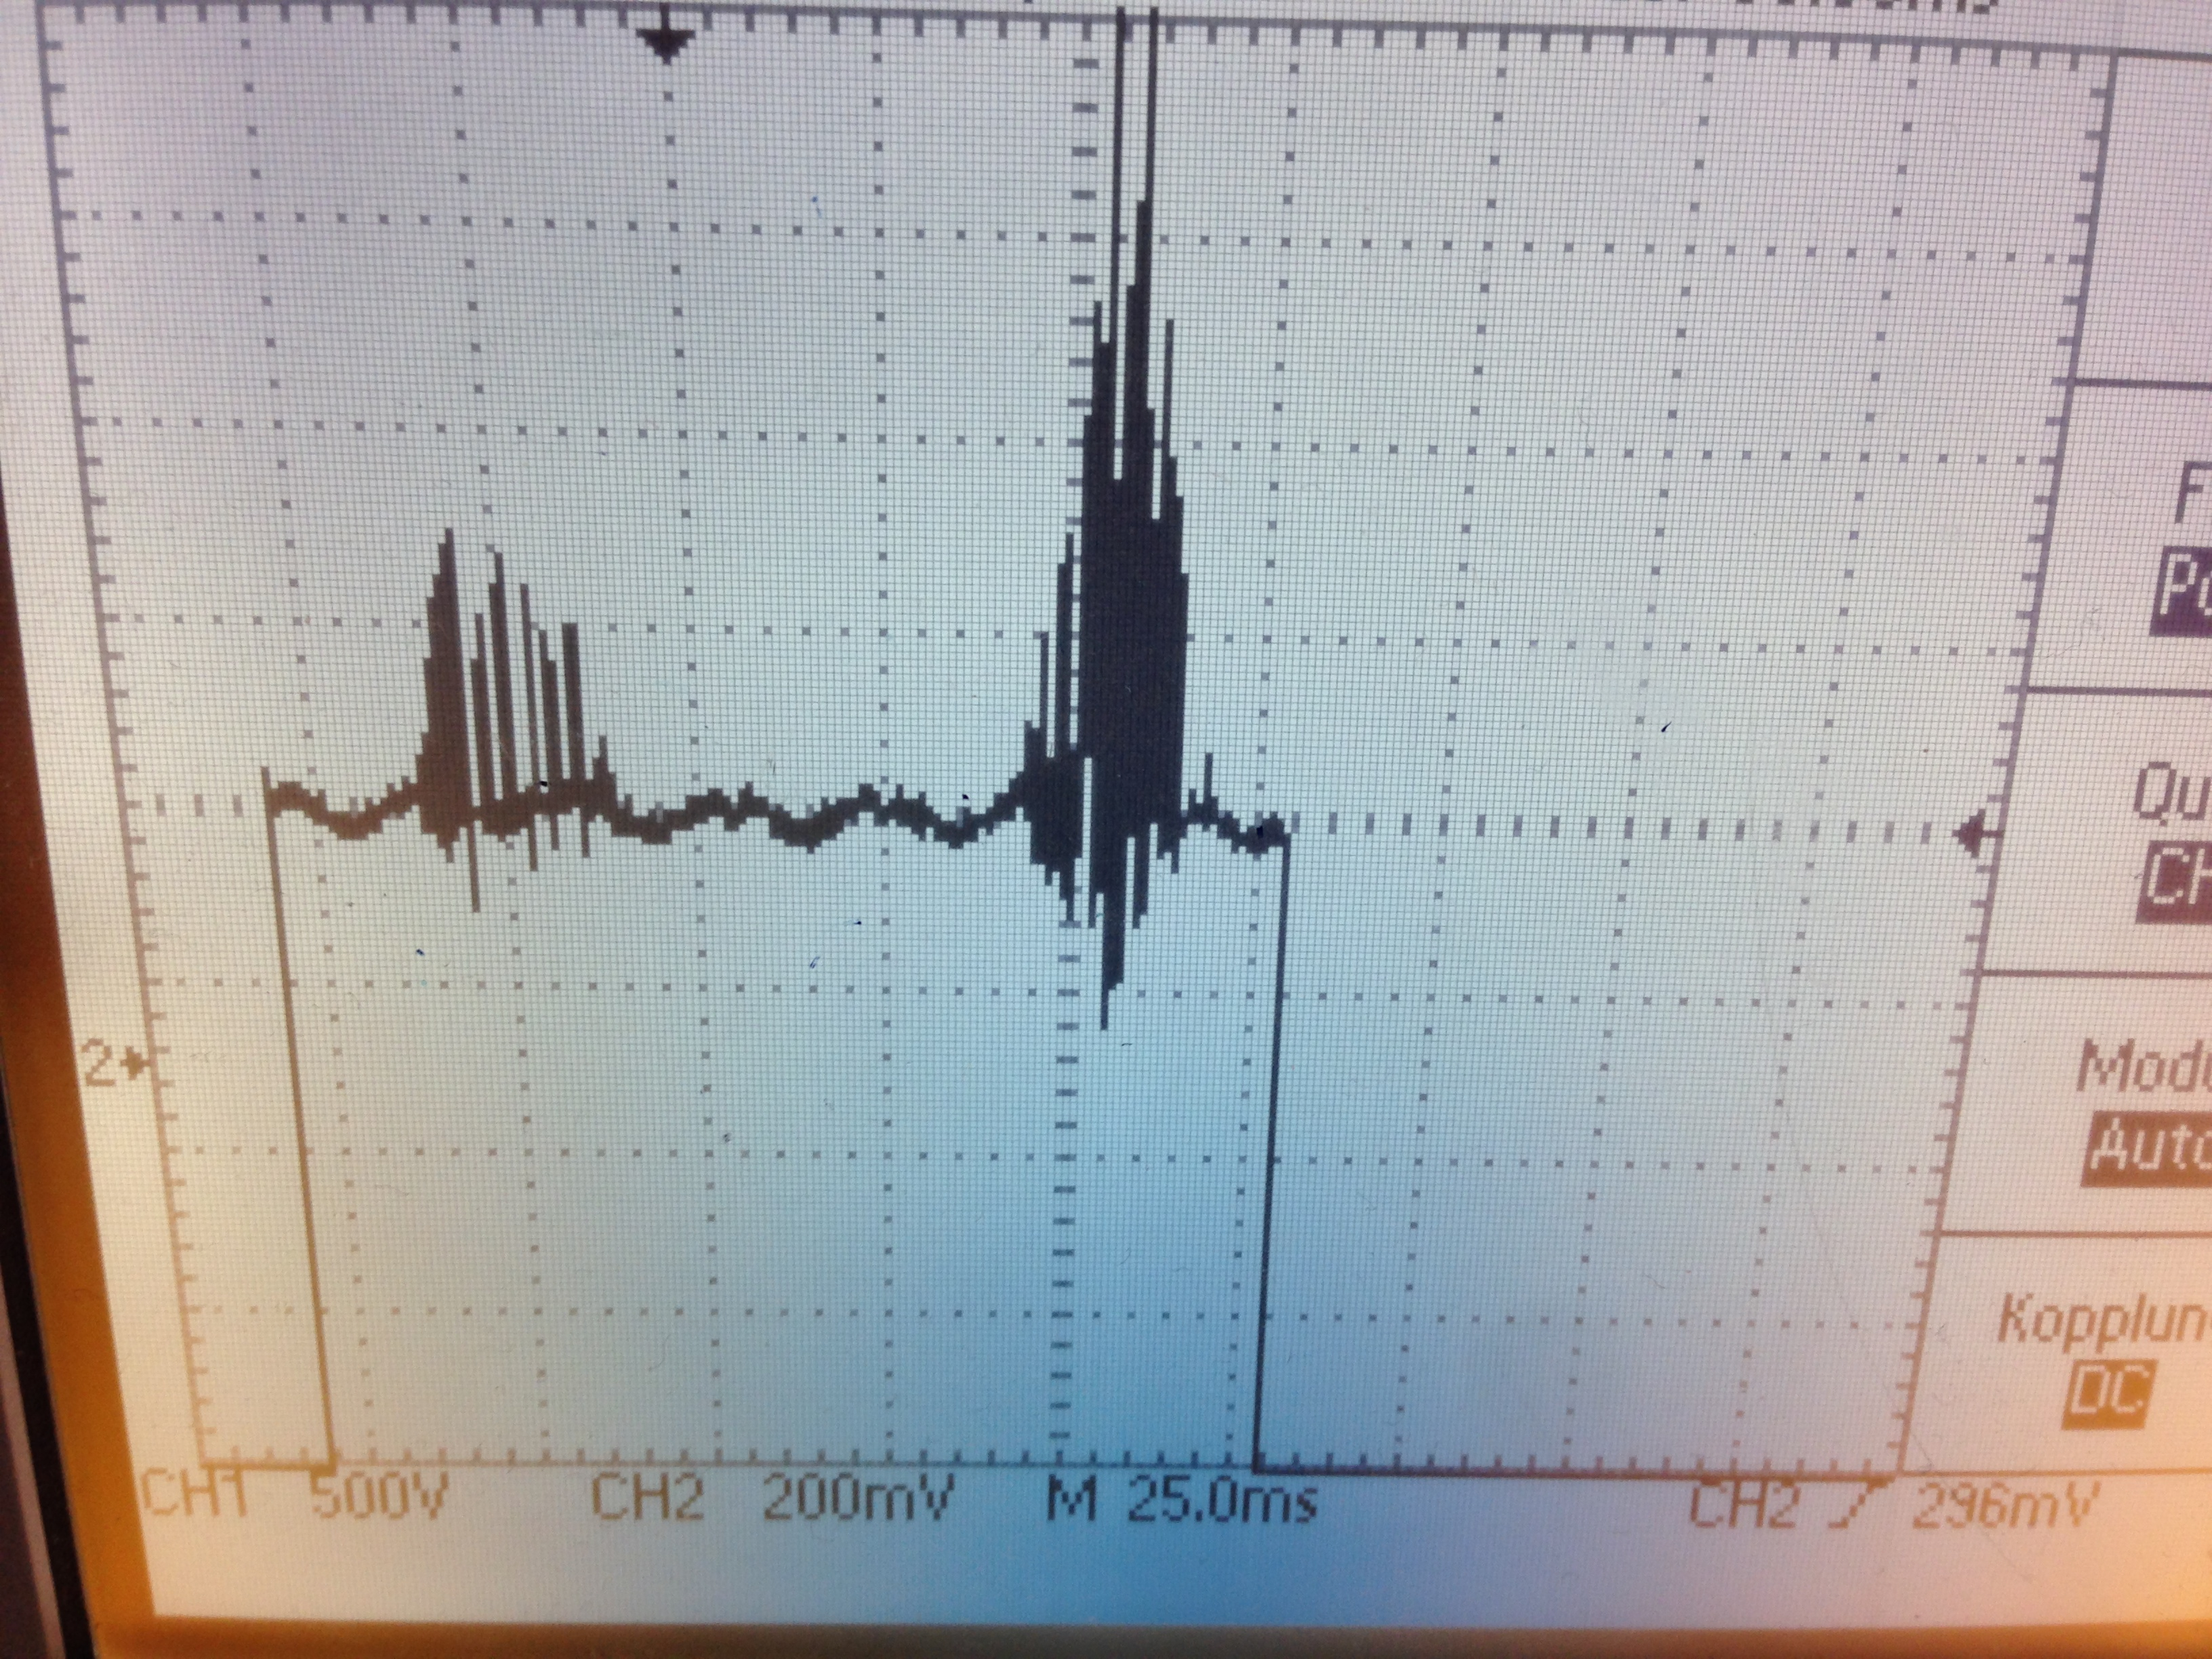
\includegraphics[scale=0.1]{img/62}
\caption{Power-Dips}
\begin{center}
\end{center}
\end{figure}

Wie in Abb. 10 dargestellt, sind nur einige Moden in einer Gaußkurve zu sehen. Wir haben diese ungefähr verlaufende Kurve zur genaueren Bestimmung der Halbwertsbreite vermessen. Wir erhielten eine Breite von (0.600 $\pm$ 0.050) GHz. Setzen wir diese in Gl. (12) zusammen mit der Masse der Neon-Atome von m = 3.35*10$^{26}$ kg und der Frequenz des Lasers von $\nu$ = 633 nm ein, so erhalten wir eine Temperatur von ca. 63.14 K. Dieser Wert ist offensichtlich unrealistisch gering. Wir sehen also, dass unsere Abschätzung der Halbwertshöhe anhand der Gaußkurve immer noch nicht gut genug war.


\end{document}
